
\begin{frame}{Symulacja robota}
%	zdjęcie Velmy w środowisku
	\begin{columns}
		\begin{column}{0.5\textwidth}
			\begin{itemize}
				\item Robot Velma - dwa manipulatory LWR Kuki, każdy o siedmiu stopniach swobody
				\item Baza mobilna - wielokierunkowa, wykorzystująca koła szwedzkie
				\item Symulacja na potrzeby prac laboratoryjnych, w początkowych fazach projektów prace na samym robocie są zbyt niebezpieczne
			\end{itemize}
		\end{column}
		\begin{column}{0.5\textwidth}
			\begin{center}
				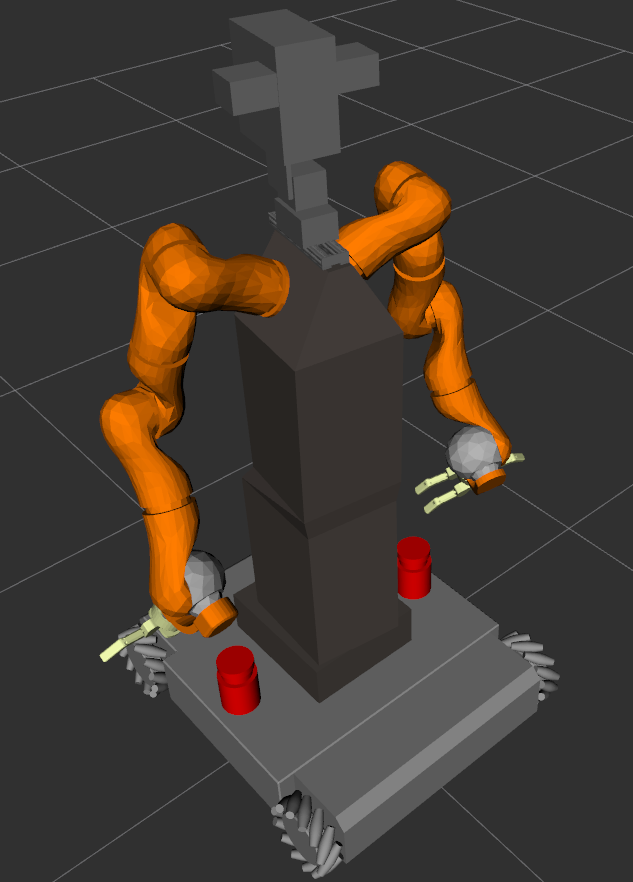
\includegraphics[height=0.7\textheight]{img/velma_wizualizacja.png} 
			\end{center}
		\end{column}		
	\end{columns}
	
\end{frame}


\begin{frame}{Symulacja części mobilnej}
	\begin{columns}
		\begin{column}{0.5\textwidth}
			\begin{center}
				MODUŁ SYMULACYJNY
			\end{center}
			\begin{itemize}
				\item kształt wizualny obiektu
				\item kolizje obiektu
				\item dynamika obiektu
			\end{itemize}
			
		\end{column}
		\begin{column}{0.5\textwidth}  %%<--- here
			\begin{center}
				MODUŁ STERUJĄCY
			\end{center}
			\begin{itemize}
				\item wykorzystuje informacje z pierwszego modułu
				\item przyjmuje jako wejście prędkość zadaną bazy
				\item oblicza siły działające na bazę
			\end{itemize}
		\end{column}
	\end{columns}
\end{frame}

\begin{frame}{Oprogramowanie części mobilnej}
	\begin{columns}
		\begin{column}{0.5\textwidth}
			\begin{center}
				ROS
			\end{center}
			\begin{itemize}
				\item popularny i rozwijany system programowania robotów
				\item umożliwia tworzenie niezależnych procesów w systemie operacyjnym komputera
				\item komunikacja między procesami z pomocą jednokierunkowych tematów i dwukierunkowych serwisów
			\end{itemize}
			
		\end{column}
		\begin{column}{0.5\textwidth}  %%<--- here
			\begin{center}
				GAZEBO
			\end{center}
			\begin{itemize}
				\item symulowanie obiektów w trzech wymiarach
				\item proste pisanie własnych pluginów w C++
				\item początkowo część ROSa, teraz niezależna platforma
			\end{itemize}
		\end{column}
	\end{columns}
\end{frame}